

\chapter{RESEARCH METHODOLOGY}

\section{Introduction}
This chapter presents the methodology for evaluating three pre-trained ASR models—OpenAI’s Whisper, Meta’s wav2vec 2.0, and Google’s CHIRP (USM)—on Japanese speech recognition. The study focuses on comparing Word Error Rate (WER) and transcription speed using formal (TED Talks) and informal (dialectal, COJADS) datasets. The chapter details the data collection, preprocessing steps (such as audio conversion and resampling), model selection rationale, and the standardized testing environment. It concludes by discussing key challenges, limitations, and ethical considerations relevant to the evaluation process.

\section{Research Design}
% This study takes a comparative approach to evaluate three ASR models that is OpenAI’s Whisper, Meta’s wav2vec 2.0, and Google’s CHIRP (USM) on formal (TED Talks) and informal (COJADS) Japanese speech. The audio data are extracted from video sources and standardized to 16 kHz, 16-bit PCM before transcription alignment. Each model is then tested in the same Hugging Face environment under identical conditions. Performance is measured primarily through Word Error Rate (WER) and transcription latency, with experiments repeated multiple times to ensure reliability. This design allows for a fair comparison of the models’ handling of different linguistic contexts and highlights potential limitations related to dataset coverage and dialectal diversity.

% student ID + name
% report
% slides
% turnitin report
% submission form
% logbook

% max 20 slide
% 7 min presentation
% 13 min Q&A

% one complete sentence before start the content of presenatation

\section{Data Collection}
\subsection{Dataset Selection}
To evaluate the performance of the models, this study will be using two source of data. The first dataset is from Ted Talk Youtube dataset which will be responsible for formal speech with clear pronunciation completes with rich and diverse vocabulary. The second dataset is the Corpus of Japanese Dialects(COJADS) which will be responsible as the input for informal speech which categorized based on regional accent and expression. The COJADS dataset only can be obtain from National Institute for Japanese Language and Linguistics (NINJAL).


\subsection{Data Pre-processing}
The pre-processing steps is the first step in doing the model comparison. This step will be tailored to prepare the datasets for input into the selected speech recognition models. For the TED Talks YouTube dataset, the audio files will be  extracted from video recordings and transcribed using Python moviepy library into Waveform Audio File Format (WAV) format. 
\begin{lstlisting}[caption={Python code to convert video to WAV format using moviepy}]
    def convert_video_to_wav(video_path, output_wav_path):
    try:
        video_clip = VideoFileClip(video_path)
        audio_path = output_wav_path\
            .replace(".wav", "_temp_audio.mp3")
        video_clip.audio.write_audiofile(audio_path)
        return audio_path
    
    except Exception as e:
        return None
\end{lstlisting}
After that, each audio file was converted to the standardized 16 kHz, 16-bit PCM format to ensure the data is compatible with the ASR models. Then the text will be manually transcribed and aligned with the corresponding audio to create accurate transcriptions for evaluation.

For the Corpus of Japanese Dialects, the data is in MP4 format and the audio files will be extracted to wav using the same method as the TED Talks YouTube dataset. Then the audio files will be resampled to resampled to the 16 kHz, 16-bit PCM format using Python pydub library.

\begin{lstlisting}[caption={Python code to resample audio to 16 kHz using pydub}]
    def resample_audio(input_audio_path, output_audio_path,\
        target_sample_rate=16000):
    try:
        audio = AudioSegment.from_file(input_audio_path)
        audio = audio.set_frame_rate(target_sample_rate)
        audio.export(output_audio_path, format="wav")
        
        print(f"Resampled audio saved to {output_audio_path}")
    except Exception as e:
        print(f"Error during audio resampling: {e}")
\end{lstlisting}
The reason for resampling the audio into 16 kHz, 16-bit PCM format is because it will align with the standard input requirements for most Automatic Speech Recognition (ASR) models. This sampling rate has the capability to capture the full frequency range of human speech, making it suitable for speech recognition tasks.


\section{Model Selection}
% this need to be detailed?
This study will be evaluating three advanced speech recognition models to determine their performance in handling the challenges of Japanese ASR. the first model is the whisper model by OpenAI is selected for its capabilities in speech-to-text transcription across diverse languages. It is also develop by OpenAI which is known for their cutting-edge research in AI and machine learning. The second model is the wav2vec 2.0 model by Meta/Facebook AI Research is chosen for its self-supervised learning approach, which reduces the dependency on large annotated datasets by leveraging unlabeled speech data. The third model is the CHIRP model by Google USM is selected for its cutting-edge multilingual capabilities, designed to handle over 100 languages with high accuracy efficiently.

\section{Model Testing and Evaluation}
\subsection{Testing Environment}
The model evaluations will be using the Hugging Face platform, which is a widely used and versatile framework for deploying and testing Machine Learning models. Hugging Face provides out of the box integration with the chosen speech recognition models. This will enable more efficient setup and execution of the testing workflows.

To provide better and more consistent evaluations, the testing environments for all models will be standardized. The sample will be prepared using the same preprocessed method for audio files which are sampled at 16 kHz and follow the 16 bit PCM standard. This will make sure all the input data will be compatible with the models Then the test will be conducted in the same environment to provide identical hardware and software configurations, so the results of the models can be compared. Each experiment will be run five times to overcome the variations in the performance of the model and the averages will be use for more accurate result.


\subsection{Performance Metrics}
To evaluate the performance of the selected speech recognition models, these key metrics will be used:

\begin{itemize}
    \item Word Error Rate: Measures the accuracy of transcriptions by calculating the percentage of words that incorrectly transcribed. This is a critical metric for assessing the overall precision of the models.
    \item Transcription Latency: Measures the time taken by each model to transcribe audio input, providing insight into their suitability for real-time applications.
    \item Handling of Formal vs. Informal Language: Evaluates how well the models perform across different linguistic contexts, including formal speech and informal, dialectal speech.
\end{itemize}

\subsection{Test Procedure}
The following step-by-step procedure was implemented to evaluate the models:

\begin{figure}[!ht]
    \centering
    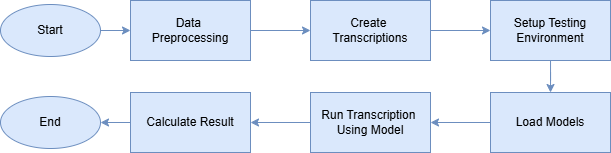
\includegraphics[width=1\textwidth]{mainmatter//images/step.png}
    \caption{Testing procedure }
\end{figure}

The model evaluation process will be start by pre-processing the audio files to ensure consistency in format. This will make sure that the audio files are compatible with the models. Then the data audio from the TED Talks YouTube dataset will be used to create transcriptions manually. The transcriptions will be aligned with the audio files to ensure accurate evaluation. The COJADS dataset did not need to be transcribed as the transcriptions are already provided. 

Then the models will be loaded into the Hugging Face platform and the preprocessed audio data will be inputted into the models one by one. The output transcriptions will be evaluated against the reference transcripts to gather the comparison metrics. The evaluation will be repeated five times for each model to ensure reliability. The average performance will be calculated for each metric to provide a more accurate representation of the models' capabilities. 

\section{Challenges and Limitations}
one significant challenge in this study is the limited availability of high-quality, annotated datasets for Japanese speech recognition. While datasets like TED Talks YouTube and the Corpus of COJADS provide valuable resources, they may not fully capture the breadth of linguistic diversity in Japanese, particularly in less-represented dialects and informal speech contexts. Additionally, variations in recording quality and noise levels within the datasets can introduce inconsistencies that may affect the models’ performance.

another limitation is the potential biases introduced by the selection of test samples. The TED Talks YouTube dataset predominantly features formal speech, which may not adequately represent everyday conversational Japanese. The Corpus of Japanese Dialects includes informal and regional speech but might not cover all dialects or account for significant inter-speaker variability. These biases could skew the evaluation results, favoring models better suited to the specific characteristics of the datasets.

\section{Ethical Considerations}
The ethical considerations of this study center on data privacy, consent, and fairness in model evaluation. The datasets used in this study contain publicly available speech recordings, ensuring that no private or sensitive information is disclosed. The TED Talks YouTube dataset and the COJADS are widely accessible and do not require individual consent for research purposes. The study will focus on evaluating the performance of speech recognition models rather than analyzing the content of the recordings, minimizing potential privacy concerns.

\section{Summary}
In this chapter, a clear research design was laid out to compare three ASR models on Japanese speech. Formal (TED Talks) and informal (COJADS) datasets were chosen for linguistic variety, and consistent preprocessing steps were described. The reasoning for selecting Whisper, wav2vec 2.0, and CHIRP (USM) was explained, followed by details on how testing will be conducted in a standardized environment to measure WER and transcription latency. Lastly, potential challenges in dataset availability, biases, and ethical considerations around data privacy were addressed.